%; whizzy chapter
% -initex iniptex -latex platex -format platex -bibtex jbibtex -fmt fmt
% 以上 whizzytex を使用する場合の設定。

%     Kansai Debian Meeting resources
%     Copyright (C) 2007 Takaya Yamashita
%     Thank you for Tokyo Debian Meeting resources

%     This program is free software; you can redistribute it and/or modify
%     it under the terms of the GNU General Public License as published by
%     the Free Software Foundation; either version 2 of the License, or
%     (at your option) any later version.

%     This program is distributed in the hope that it will be useful,
%     but WITHOUT ANY WARRANTY; without even the implied warranty of
%     MERCHANTABILITY or FITNESS FOR A PARTICULAR PURPOSE.  See the
%     GNU General Public License for more details.

%     You should have received a copy of the GNU General Public License
%     along with this program; if not, write to the Free Software
%     Foundation, Inc., 51 Franklin St, Fifth Floor, Boston, MA  02110-1301 USA

%  preview (shell-command (concat "evince " (replace-regexp-in-string "tex$" "pdf"(buffer-file-name)) "&"))
% 画像ファイルを処理するためにはebbを利用してboundingboxを作成。
%(shell-command "cd image200708; ebb *.png")

%%ここからヘッダ開始。

\documentclass[mingoth,a4paper]{jsarticle}
\usepackage{kansaimonthlyreport}
\usepackage{ascmac}

\begin{document}
\begin{commandline}
    27	%%ここからヘッダ開始。
    28	
    29	\documentclass[mingoth,a4paper]{jsarticle}
    30	\usepackage{kansaimonthlyreport}
    31	\usepackage{ascmac}
    32	
    33	% 日付を定義する、毎月変わります。
    34	\newcommand{\debmtgyear}{2008}
    35	\newcommand{\debmtgdate}{23}
    36	\newcommand{\debmtgmonth}{2}
    37	\newcommand{\debmtgnumber}{10}
    38	
    39	\begin{document}
    40	
    41	\begin{titlepage}
    42	
    43	% 毎月変更する部分, 本文の末尾も修正することをわすれずに
    44	
    45	 第\debmtgnumber{}回 関西 Debian 勉強会資料
    46	
    47	\vspace{2cm}
    48	
    49	\begin{center}
    50	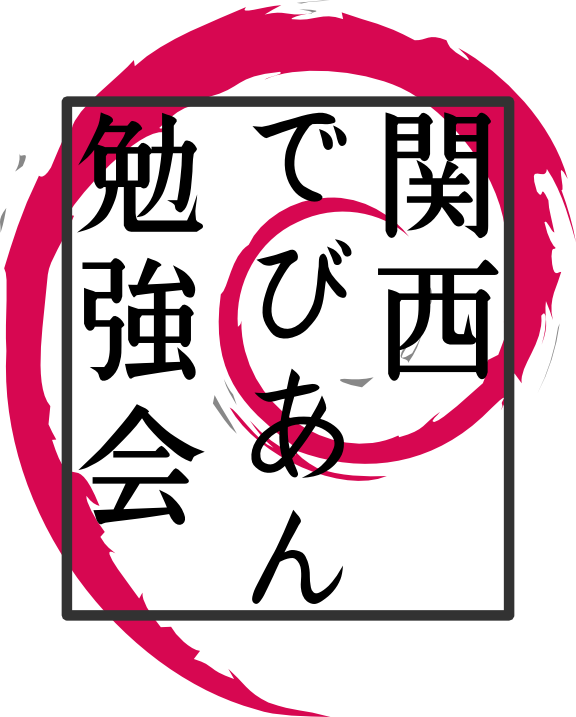
\includegraphics{image200802/kansaidebianlogo.png}
    51	\end{center}
    52	
    53	\begin{flushright}
    54	\hfill{}関西 Debian 勉強会担当者 山下 尊也\\
    55	\hfill{}\debmtgyear{}年\debmtgmonth{}月\debmtgdate{}日
    56	\end{flushright}
    57	
    58	\thispagestyle{empty}
    59	\end{titlepage}
    60	
    61	\dancersection{Introduction}{山下 尊也}
    62	 
    63	 関西 Debian 勉強会はDebian GNU/Linux のさまざ
    64	 まなトピック(新しいパッケージ、Debian 特有の機能の仕組、Debian 界隈で起
    65	 こった出来事、などなど)について話し合う会です。
    66	
    67	 目的として次の三つを考えています。
    68	 \begin{itemize}
    69	  \item MLや掲示板ではなく、直接顔を合わせる事での情報交換の促進
    70	  \item 定期的に集まれる場所
    71	  \item 資料の作成
    72	 \end{itemize}
    73	
    74	 それでは、楽しい一時をお楽しみ下さい。
    75	
    76	\newpage
略
    92	\dancersection{GIS on Debian GNU/Linux!}{清野 陽一}
    93	
    94	\subsection{はじめに}
    95	\subsubsection{社会的整備の進展}
    96	
    97	\begin{itemize}
    98	 \item 国際情勢
    99	       \begin{itemize}
   100		\item 地図情報を電子化して扱おうという試みは1960年代ごろから始まってい
   101		      る。当初は研究目的。
   102		\item メインフレーム上ではなく、ワークステーションやパーソナルコンピュー
   103		      タの発達に伴い、1980年代頃からこれらのコンピュータ上で動かせるシ
   104		      ステムが普及し始める。
   105		\item 後述する地上観測衛星(ランドサット衛星1号機の打ち上げは1972年)や
   106		      スペースシャトルの運用により、リモートセンシングなどの活用が1970
   107		      年代より行われるようになる。
   108	       \end{itemize}
   109	 \item 日本国内
   110	 \begin{itemize}
   111	  \item 行政サイド \\
   112		日本においては、国土に関する数値情報の電子化
   113		\begin{quotation}
   114		 「平成7年1月の阪神・
   115		 淡路大震災の反省等をきっかけに、政府において、GISに関する本格的な
   116		 取組が始まった。」(国土地理院
   117		 GIS(\url{http://www.gsi.go.jp/GIS/whatisgis.html})による) 
   118		\end{quotation}
   119		→国を挙げての政策実施。2002年の小泉内閣における「e-Japan重点計
   120		画-2002」の重点政策のうち、4番目の「行政の情報化及び公共分野にお
   121		ける情報通信技術の活用の推進」においてGISの推進が盛り込まれる。
   122		ex)国土地理院の数値地図(CD-ROM版)は平成9(1997)年頃から整備される
   123		ようになってきている。
   124	  \item 建設サイド
   125		\begin{itemize}
   126		 \item CAD(Computer Aided Design)の普及
   127		 \item 電子納品・標準化
   128		 \item 建設省・国土交通省の後押し
   129		\end{itemize}
   130	 \end{itemize}
   131	\end{itemize}
\end{commandline}
\end{document}
